% Options for packages loaded elsewhere
\PassOptionsToPackage{unicode}{hyperref}
\PassOptionsToPackage{hyphens}{url}
%
\documentclass[
]{article}
\usepackage{amsmath,amssymb}
\usepackage{lmodern}
\usepackage{ifxetex,ifluatex}
\ifnum 0\ifxetex 1\fi\ifluatex 1\fi=0 % if pdftex
  \usepackage[T1]{fontenc}
  \usepackage[utf8]{inputenc}
  \usepackage{textcomp} % provide euro and other symbols
\else % if luatex or xetex
  \usepackage{unicode-math}
  \defaultfontfeatures{Scale=MatchLowercase}
  \defaultfontfeatures[\rmfamily]{Ligatures=TeX,Scale=1}
\fi
% Use upquote if available, for straight quotes in verbatim environments
\IfFileExists{upquote.sty}{\usepackage{upquote}}{}
\IfFileExists{microtype.sty}{% use microtype if available
  \usepackage[]{microtype}
  \UseMicrotypeSet[protrusion]{basicmath} % disable protrusion for tt fonts
}{}
\makeatletter
\@ifundefined{KOMAClassName}{% if non-KOMA class
  \IfFileExists{parskip.sty}{%
    \usepackage{parskip}
  }{% else
    \setlength{\parindent}{0pt}
    \setlength{\parskip}{6pt plus 2pt minus 1pt}}
}{% if KOMA class
  \KOMAoptions{parskip=half}}
\makeatother
\usepackage{xcolor}
\IfFileExists{xurl.sty}{\usepackage{xurl}}{} % add URL line breaks if available
\IfFileExists{bookmark.sty}{\usepackage{bookmark}}{\usepackage{hyperref}}
\hypersetup{
  pdftitle={semana 4},
  pdfauthor={luis},
  hidelinks,
  pdfcreator={LaTeX via pandoc}}
\urlstyle{same} % disable monospaced font for URLs
\usepackage[margin=1in]{geometry}
\usepackage{color}
\usepackage{fancyvrb}
\newcommand{\VerbBar}{|}
\newcommand{\VERB}{\Verb[commandchars=\\\{\}]}
\DefineVerbatimEnvironment{Highlighting}{Verbatim}{commandchars=\\\{\}}
% Add ',fontsize=\small' for more characters per line
\usepackage{framed}
\definecolor{shadecolor}{RGB}{248,248,248}
\newenvironment{Shaded}{\begin{snugshade}}{\end{snugshade}}
\newcommand{\AlertTok}[1]{\textcolor[rgb]{0.94,0.16,0.16}{#1}}
\newcommand{\AnnotationTok}[1]{\textcolor[rgb]{0.56,0.35,0.01}{\textbf{\textit{#1}}}}
\newcommand{\AttributeTok}[1]{\textcolor[rgb]{0.77,0.63,0.00}{#1}}
\newcommand{\BaseNTok}[1]{\textcolor[rgb]{0.00,0.00,0.81}{#1}}
\newcommand{\BuiltInTok}[1]{#1}
\newcommand{\CharTok}[1]{\textcolor[rgb]{0.31,0.60,0.02}{#1}}
\newcommand{\CommentTok}[1]{\textcolor[rgb]{0.56,0.35,0.01}{\textit{#1}}}
\newcommand{\CommentVarTok}[1]{\textcolor[rgb]{0.56,0.35,0.01}{\textbf{\textit{#1}}}}
\newcommand{\ConstantTok}[1]{\textcolor[rgb]{0.00,0.00,0.00}{#1}}
\newcommand{\ControlFlowTok}[1]{\textcolor[rgb]{0.13,0.29,0.53}{\textbf{#1}}}
\newcommand{\DataTypeTok}[1]{\textcolor[rgb]{0.13,0.29,0.53}{#1}}
\newcommand{\DecValTok}[1]{\textcolor[rgb]{0.00,0.00,0.81}{#1}}
\newcommand{\DocumentationTok}[1]{\textcolor[rgb]{0.56,0.35,0.01}{\textbf{\textit{#1}}}}
\newcommand{\ErrorTok}[1]{\textcolor[rgb]{0.64,0.00,0.00}{\textbf{#1}}}
\newcommand{\ExtensionTok}[1]{#1}
\newcommand{\FloatTok}[1]{\textcolor[rgb]{0.00,0.00,0.81}{#1}}
\newcommand{\FunctionTok}[1]{\textcolor[rgb]{0.00,0.00,0.00}{#1}}
\newcommand{\ImportTok}[1]{#1}
\newcommand{\InformationTok}[1]{\textcolor[rgb]{0.56,0.35,0.01}{\textbf{\textit{#1}}}}
\newcommand{\KeywordTok}[1]{\textcolor[rgb]{0.13,0.29,0.53}{\textbf{#1}}}
\newcommand{\NormalTok}[1]{#1}
\newcommand{\OperatorTok}[1]{\textcolor[rgb]{0.81,0.36,0.00}{\textbf{#1}}}
\newcommand{\OtherTok}[1]{\textcolor[rgb]{0.56,0.35,0.01}{#1}}
\newcommand{\PreprocessorTok}[1]{\textcolor[rgb]{0.56,0.35,0.01}{\textit{#1}}}
\newcommand{\RegionMarkerTok}[1]{#1}
\newcommand{\SpecialCharTok}[1]{\textcolor[rgb]{0.00,0.00,0.00}{#1}}
\newcommand{\SpecialStringTok}[1]{\textcolor[rgb]{0.31,0.60,0.02}{#1}}
\newcommand{\StringTok}[1]{\textcolor[rgb]{0.31,0.60,0.02}{#1}}
\newcommand{\VariableTok}[1]{\textcolor[rgb]{0.00,0.00,0.00}{#1}}
\newcommand{\VerbatimStringTok}[1]{\textcolor[rgb]{0.31,0.60,0.02}{#1}}
\newcommand{\WarningTok}[1]{\textcolor[rgb]{0.56,0.35,0.01}{\textbf{\textit{#1}}}}
\usepackage{graphicx}
\makeatletter
\def\maxwidth{\ifdim\Gin@nat@width>\linewidth\linewidth\else\Gin@nat@width\fi}
\def\maxheight{\ifdim\Gin@nat@height>\textheight\textheight\else\Gin@nat@height\fi}
\makeatother
% Scale images if necessary, so that they will not overflow the page
% margins by default, and it is still possible to overwrite the defaults
% using explicit options in \includegraphics[width, height, ...]{}
\setkeys{Gin}{width=\maxwidth,height=\maxheight,keepaspectratio}
% Set default figure placement to htbp
\makeatletter
\def\fps@figure{htbp}
\makeatother
\setlength{\emergencystretch}{3em} % prevent overfull lines
\providecommand{\tightlist}{%
  \setlength{\itemsep}{0pt}\setlength{\parskip}{0pt}}
\setcounter{secnumdepth}{-\maxdimen} % remove section numbering
\ifluatex
  \usepackage{selnolig}  % disable illegal ligatures
\fi

\title{semana 4}
\author{luis}
\date{19/7/2021}

\begin{document}
\maketitle

\tableofcontents

\hypertarget{regresiuxf3n-regularizada}{%
\section{Regresión regularizada}\label{regresiuxf3n-regularizada}}

\emph{Idea básica}

\begin{enumerate}
\def\labelenumi{\arabic{enumi}.}
\tightlist
\item
  Ajustar un modelo de regresión
\item
  Penalizar (o reducir) los coeficientes grandes
\end{enumerate}

\textbf{Pros: }

\begin{itemize}
\tightlist
\item
  Puede ayudar con la compensación de sesgo / varianza
\item
  Puede ayudar con la selección del modelo
\end{itemize}

\textbf{Contras:}

\begin{itemize}
\tightlist
\item
  Puede ser computacionalmente exigente en grandes conjuntos de datos
\item
  No funciona tan bien como bosques random forests y boosting.
\end{itemize}

ejemplo motivacional:

\[Y = \beta_0 + \beta_1 X_1 + \beta_2 X_2 + \epsilon\]

donde \(X_1\) y \(X_2\) están casi perfectamente correlacionados
(colineales). Puede aproximar este modelo por:

\[Y = \beta_0 + (\beta_1 + \beta_2)X_1 + \epsilon\]

El resultado es:

\begin{itemize}
\tightlist
\item
  Obtendrá una buena estimación de \(Y\)
\item
  La estimación (de \(Y\)) estará sesgada
\item
  Podemos reducir la variación en la estimación.
\end{itemize}

con datos de cancer de prostata

\begin{Shaded}
\begin{Highlighting}[]
\FunctionTok{library}\NormalTok{(ElemStatLearn); }\FunctionTok{data}\NormalTok{(prostate)}
\FunctionTok{str}\NormalTok{(prostate)}
\end{Highlighting}
\end{Shaded}

\begin{verbatim}
## 'data.frame':    97 obs. of  10 variables:
##  $ lcavol : num  -0.58 -0.994 -0.511 -1.204 0.751 ...
##  $ lweight: num  2.77 3.32 2.69 3.28 3.43 ...
##  $ age    : int  50 58 74 58 62 50 64 58 47 63 ...
##  $ lbph   : num  -1.39 -1.39 -1.39 -1.39 -1.39 ...
##  $ svi    : int  0 0 0 0 0 0 0 0 0 0 ...
##  $ lcp    : num  -1.39 -1.39 -1.39 -1.39 -1.39 ...
##  $ gleason: int  6 6 7 6 6 6 6 6 6 6 ...
##  $ pgg45  : int  0 0 20 0 0 0 0 0 0 0 ...
##  $ lpsa   : num  -0.431 -0.163 -0.163 -0.163 0.372 ...
##  $ train  : logi  TRUE TRUE TRUE TRUE TRUE TRUE ...
\end{verbatim}

podemos ver que llega un punto en que el error aumenta si aumenta el
número de variables

\begin{center}\includegraphics[width=1\linewidth]{D:/luism/Documents/courses/assets/img/prostate} \end{center}

entonces el patron mas comun es

\begin{center}\includegraphics[width=1\linewidth]{D:/luism/Documents/courses/assets/img/trainingandtest} \end{center}

Enfoque de selección de modelos: muestras divididas

\begin{itemize}
\tightlist
\item
  Acercarse

  \begin{enumerate}
  \def\labelenumi{\arabic{enumi}.}
  \tightlist
  \item
    Divida los datos en entrenamiento / prueba / validación
  \item
    Trate la validación como datos de prueba, entrene todos los modelos
    competidores en los datos del train y elija el mejor para la
    validación.
  \item
    Para evaluar adecuadamente el rendimiento sobre nuevos datos,
    aplique al conjunto de prueba.
  \item
    Puede volver a dividir y volver a realizar los pasos 1-3
  \end{enumerate}
\item
  Dos problemas comunes

  \begin{itemize}
  \tightlist
  \item
    Datos limitados
  \item
    Complejidad computacional
  \end{itemize}
\end{itemize}

\url{http://www.biostat.jhsph.edu/~ririzarr/Teaching/649/}
\url{http://www.cbcb.umd.edu/~hcorrada/PracticalML/}

\emph{descomposición de Error de predicción esperado}

sea \(Y_i = f(X_i) + \epsilon_i\)

\(EPE(\lambda) = E\left[\{Y - \hat{f}_{\lambda}(X)\}^2\right]\)

supongamos que \(\hat{f}_{\lambda}\) es la estimación de los datos de
entrenamiento y mira un nuevo punto de datos \(X = x^*\)

\[E\left[\{Y - \hat{f}_{\lambda}(x^*)\}^2\right] = \sigma^2 + \{E[\hat{f}_{\lambda}(x^*)] - f(x^*)\}^2 + var[\hat{f}_\lambda(x_0)]\]

\begin{center}
= Error irreducible + sesgo$^2$ + varianza
\end{center}

\emph{Umbral duro}

\begin{itemize}
\item
  Modelo \(Y = f (X) + \epsilon\)
\item
  Establecer \(\hat {f} _ {\lambda} (x) = x '\beta\)
\item
  Restrinja solo los coeficientes \(\lambda\) para que sean distintos de
  cero.
\item
  El problema de selección es después de elegir \(\lambda\) averiguar
  qué coeficientes \(p - \lambda\) hacen distintos de cero
\end{itemize}

\emph{Regularización para regresión}

Si los \(\beta_j\) no están restringidos: * Pueden explotar * Y, por
tanto, son susceptibles a variaciones muy elevadas

Para controlar la varianza, podríamos regularizar/reducir los
coeficientes.

\[PRSS(\beta) = \sum_{j=1}^n (Y_j - \sum_{i=1}^m \beta_{1i} X_{ij})^2 + P(\lambda; \beta)\]
donde \(PRSS\) es una forma penalizada de la suma de cuadrados. Cosas
que se buscan comúnmente

\begin{itemize}
\tightlist
\item
  La penalización reduce la complejidad
\item
  La penalización reduce la varianza
\item
  La penalización respeta la estructura del problema.
\end{itemize}

\hypertarget{regresion-ridge}{%
\subsection{Regresion Ridge}\label{regresion-ridge}}

Resuelve:

\[\sum_{i=1}^N \left(y_i - \beta_0 + \sum_{j=1}^p x_{ij}\beta_j \right)^2 + \lambda \sum_{j=1}^p \beta_j^2\]
equivalente a resolver

\(\sum_{i=1}^N \left(y_i - \beta_0 + \sum_{j=1}^p x_{ij}\beta_j \right)^2\)
sujeto a \(\sum_{j=1}^p \beta_j^2 \leq s\) donde \(s\) es inversamente
proporcional a \(\lambda\)

La inclusión de \(\lambda\) hace que el problema no sea singular incluso
si \(X ^ TX\) no es invertible.

trayectorias de los coeficentes al aumentar \(\lambda\)

\begin{center}\includegraphics[width=1\linewidth]{D:/luism/Documents/courses/assets/img/ridgepath} \end{center}

Parámetro de ajuste \(\lambda\)

\begin{itemize}
\tightlist
\item
  \(\lambda\) controla el tamaño de los coeficientes
\item
  \(\lambda\) controla la cantidad de regularización \{\bf\}
\item
  cuando \(\lambda\rightarrow 0\) obtenemos la solución de mínimos
  cuadrados
\item
  cuando \(\lambda\rightarrow \infty\) tenemos
  \(\hat {\beta} _ {\lambda = \infty} ^ {ridge} = 0\)
\end{itemize}

\hypertarget{regresion-lasso}{%
\subsection{regresion lasso}\label{regresion-lasso}}

\(\sum_{i=1}^N \left(y_i - \beta_0 + \sum_{j=1}^p x_{ij}\beta_j \right)^2\)
sujeto a \(\sum_{j=1}^p |\beta_j| \leq s\)

equivalente a

\[\sum_{i=1}^N \left(y_i - \beta_0 + \sum_{j=1}^p x_{ij}\beta_j \right)^2 + \lambda \sum_{j=1}^p |\beta_j|\]
Para matrices de diseño ortonormal (¡no la norma!), Esto tiene una
solución de forma cerrada

\[\hat{\beta}_j = sign(\hat{\beta}_j^0)(|\hat{\beta}_j^0 - \gamma)^{+}\]

but not in general.

\url{http://www.biostat.jhsph.edu/~ririzarr/Teaching/649/}
\url{http://www.cbcb.umd.edu/~hcorrada/PracticalML/}

\hypertarget{notas-y-futuras-lecturas}{%
\subsection{Notas y futuras lecturas}\label{notas-y-futuras-lecturas}}

\begin{itemize}
\tightlist
\item
  \href{http://www.cbcb.umd.edu/~hcorrada/PracticalML/}{Hector Corrada
  Bravo's Practical Machine Learning lecture notes}
\item
  \href{http://www.cbcb.umd.edu/~hcorrada/AMSC689.html\#readings}{Hector's
  penalized regression reading list}
\item
  \href{http://statweb.stanford.edu/~tibs/ElemStatLearn/}{Elements of
  Statistical Learning}
\item
  In \texttt{caret} methods are:

  \begin{itemize}
  \tightlist
  \item
    \texttt{ridge}
  \item
    \texttt{lasso}
  \item
    \texttt{relaxo}
  \end{itemize}
\end{itemize}

\hypertarget{combinando-predictores}{%
\section{combinando predictores}\label{combinando-predictores}}

Ideas claves

\begin{itemize}
\tightlist
\item
  Puede combinar clasificadores promediando / votando
\item
  La combinación de clasificadores mejora la precisión
\item
  La combinación de clasificadores reduce la interpretabilidad.
\item
  Boosting, bagging, y random forests son variantes de este tema.
\end{itemize}

\_Supongamos que tenemos 5 clasificadores completamente independientes

Si la precisión es del 70\% para cada uno: *
\(10\times(0.7)^3(0.3)^2+5\times(0.7)^4(0.3)^2+(0.7)^5\) * 83,7\% de
precisión del voto mayoritario

Con 101 clasificadores independientes * 99,9\% de precisión del voto
mayoritario\_

\href{https://github.com/lgreski/datasciencectacontent/blob/master/markdown/pml-combiningPredictorsBinomial.md}{como
se calculo}

\emph{Enfoques para combinar clasificadores}

\begin{enumerate}
\def\labelenumi{\arabic{enumi}.}
\tightlist
\item
  Bagging, boosting, random forests
\end{enumerate}

\begin{itemize}
\tightlist
\item
  Suelen combinar clasificadores similares
\end{itemize}

\begin{enumerate}
\def\labelenumi{\arabic{enumi}.}
\setcounter{enumi}{1}
\tightlist
\item
  Combinando diferentes clasificadores

  \begin{itemize}
  \tightlist
  \item
    Modelo de apilamiento (stacking)
  \item
    Modelos de ensamble (ensembling)
  \end{itemize}
\end{enumerate}

ejemplo con datos wage

\textbf{creando conjuntos de training, test y validation}

\begin{Shaded}
\begin{Highlighting}[]
\FunctionTok{library}\NormalTok{(ISLR); }\FunctionTok{data}\NormalTok{(Wage); }\FunctionTok{library}\NormalTok{(ggplot2); }\FunctionTok{library}\NormalTok{(caret);}
\NormalTok{Wage }\OtherTok{\textless{}{-}} \FunctionTok{subset}\NormalTok{(Wage,}\AttributeTok{select=}\SpecialCharTok{{-}}\FunctionTok{c}\NormalTok{(logwage))}

\CommentTok{\# Create a building data set and validation set}
\NormalTok{inBuild }\OtherTok{\textless{}{-}} \FunctionTok{createDataPartition}\NormalTok{(}\AttributeTok{y=}\NormalTok{Wage}\SpecialCharTok{$}\NormalTok{wage,}
                              \AttributeTok{p=}\FloatTok{0.7}\NormalTok{, }\AttributeTok{list=}\ConstantTok{FALSE}\NormalTok{)}
\NormalTok{validation }\OtherTok{\textless{}{-}}\NormalTok{ Wage[}\SpecialCharTok{{-}}\NormalTok{inBuild,]; buildData }\OtherTok{\textless{}{-}}\NormalTok{ Wage[inBuild,]}

\NormalTok{inTrain }\OtherTok{\textless{}{-}} \FunctionTok{createDataPartition}\NormalTok{(}\AttributeTok{y=}\NormalTok{buildData}\SpecialCharTok{$}\NormalTok{wage,}
                              \AttributeTok{p=}\FloatTok{0.7}\NormalTok{, }\AttributeTok{list=}\ConstantTok{FALSE}\NormalTok{)}
\NormalTok{training }\OtherTok{\textless{}{-}}\NormalTok{ buildData[inTrain,]; testing }\OtherTok{\textless{}{-}}\NormalTok{ buildData[}\SpecialCharTok{{-}}\NormalTok{inTrain,]}

\FunctionTok{dim}\NormalTok{(training)}
\end{Highlighting}
\end{Shaded}

\begin{verbatim}
## [1] 1474   10
\end{verbatim}

\begin{Shaded}
\begin{Highlighting}[]
\FunctionTok{dim}\NormalTok{(testing)}
\end{Highlighting}
\end{Shaded}

\begin{verbatim}
## [1] 628  10
\end{verbatim}

\begin{Shaded}
\begin{Highlighting}[]
\FunctionTok{dim}\NormalTok{(validation)}
\end{Highlighting}
\end{Shaded}

\begin{verbatim}
## [1] 898  10
\end{verbatim}

despues creamos 2 diferentes modelos

\begin{Shaded}
\begin{Highlighting}[]
\NormalTok{mod1 }\OtherTok{\textless{}{-}} \FunctionTok{train}\NormalTok{(wage }\SpecialCharTok{\textasciitilde{}}\NormalTok{.,}\AttributeTok{method=}\StringTok{"glm"}\NormalTok{,}\AttributeTok{data=}\NormalTok{training)}
\NormalTok{mod2 }\OtherTok{\textless{}{-}} \FunctionTok{train}\NormalTok{(wage }\SpecialCharTok{\textasciitilde{}}\NormalTok{.,}\AttributeTok{method=}\StringTok{"rf"}\NormalTok{,}
              \AttributeTok{data=}\NormalTok{training, }
              \AttributeTok{trControl =} \FunctionTok{trainControl}\NormalTok{(}\AttributeTok{method=}\StringTok{"cv"}\NormalTok{),}\AttributeTok{number=}\DecValTok{3}\NormalTok{)}
\end{Highlighting}
\end{Shaded}

luego predecimos en el connjunto de testing, por el color vemos que no
funciona del todo bien

\begin{Shaded}
\begin{Highlighting}[]
\NormalTok{pred1 }\OtherTok{\textless{}{-}} \FunctionTok{predict}\NormalTok{(mod1,testing); pred2 }\OtherTok{\textless{}{-}} \FunctionTok{predict}\NormalTok{(mod2,testing)}
\FunctionTok{qplot}\NormalTok{(pred1,pred2,}\AttributeTok{colour=}\NormalTok{wage,}\AttributeTok{data=}\NormalTok{testing)}
\end{Highlighting}
\end{Shaded}

\begin{center}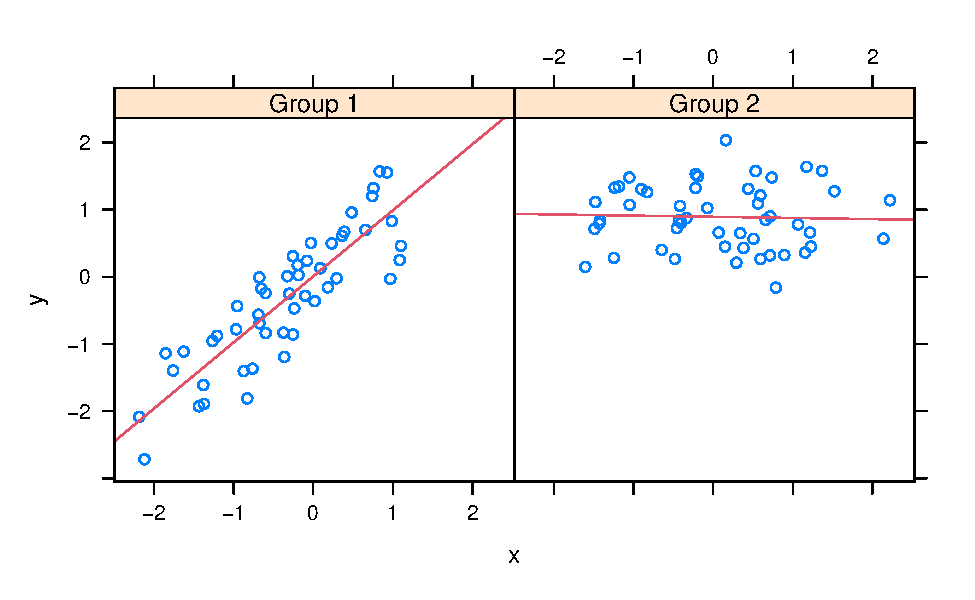
\includegraphics{semana_4_files/figure-latex/unnamed-chunk-6-1} \end{center}

ahora construimos un modelos que combine los dos predictores

\begin{Shaded}
\begin{Highlighting}[]
\NormalTok{predDF }\OtherTok{\textless{}{-}} \FunctionTok{data.frame}\NormalTok{(pred1,pred2,}\AttributeTok{wage=}\NormalTok{testing}\SpecialCharTok{$}\NormalTok{wage)}
\NormalTok{combModFit }\OtherTok{\textless{}{-}} \FunctionTok{train}\NormalTok{(wage }\SpecialCharTok{\textasciitilde{}}\NormalTok{.,}\AttributeTok{method=}\StringTok{"gam"}\NormalTok{,}\AttributeTok{data=}\NormalTok{predDF)}
\NormalTok{combPred }\OtherTok{\textless{}{-}} \FunctionTok{predict}\NormalTok{(combModFit,predDF)}
\end{Highlighting}
\end{Shaded}

errores en testing

\begin{Shaded}
\begin{Highlighting}[]
\FunctionTok{sqrt}\NormalTok{(}\FunctionTok{sum}\NormalTok{((pred1}\SpecialCharTok{{-}}\NormalTok{testing}\SpecialCharTok{$}\NormalTok{wage)}\SpecialCharTok{\^{}}\DecValTok{2}\NormalTok{))}
\end{Highlighting}
\end{Shaded}

\begin{verbatim}
## [1] 858.4733
\end{verbatim}

\begin{Shaded}
\begin{Highlighting}[]
\FunctionTok{sqrt}\NormalTok{(}\FunctionTok{sum}\NormalTok{((pred2}\SpecialCharTok{{-}}\NormalTok{testing}\SpecialCharTok{$}\NormalTok{wage)}\SpecialCharTok{\^{}}\DecValTok{2}\NormalTok{))}
\end{Highlighting}
\end{Shaded}

\begin{verbatim}
## [1] 888.5931
\end{verbatim}

\begin{Shaded}
\begin{Highlighting}[]
\FunctionTok{sqrt}\NormalTok{(}\FunctionTok{sum}\NormalTok{((combPred}\SpecialCharTok{{-}}\NormalTok{testing}\SpecialCharTok{$}\NormalTok{wage)}\SpecialCharTok{\^{}}\DecValTok{2}\NormalTok{))}
\end{Highlighting}
\end{Shaded}

\begin{verbatim}
## [1] 841.6465
\end{verbatim}

prediciendo en el conjunto de validacion

\begin{Shaded}
\begin{Highlighting}[]
\NormalTok{pred1V }\OtherTok{\textless{}{-}} \FunctionTok{predict}\NormalTok{(mod1,validation); pred2V }\OtherTok{\textless{}{-}} \FunctionTok{predict}\NormalTok{(mod2,validation)}
\NormalTok{predVDF }\OtherTok{\textless{}{-}} \FunctionTok{data.frame}\NormalTok{(}\AttributeTok{pred1=}\NormalTok{pred1V,}\AttributeTok{pred2=}\NormalTok{pred2V)}
\NormalTok{combPredV }\OtherTok{\textless{}{-}} \FunctionTok{predict}\NormalTok{(combModFit,predVDF)}
\end{Highlighting}
\end{Shaded}

evaluando en validacion

\begin{Shaded}
\begin{Highlighting}[]
\FunctionTok{sqrt}\NormalTok{(}\FunctionTok{sum}\NormalTok{((pred1V}\SpecialCharTok{{-}}\NormalTok{validation}\SpecialCharTok{$}\NormalTok{wage)}\SpecialCharTok{\^{}}\DecValTok{2}\NormalTok{))}
\end{Highlighting}
\end{Shaded}

\begin{verbatim}
## [1] 1028.13
\end{verbatim}

\begin{Shaded}
\begin{Highlighting}[]
\FunctionTok{sqrt}\NormalTok{(}\FunctionTok{sum}\NormalTok{((pred2V}\SpecialCharTok{{-}}\NormalTok{validation}\SpecialCharTok{$}\NormalTok{wage)}\SpecialCharTok{\^{}}\DecValTok{2}\NormalTok{))}
\end{Highlighting}
\end{Shaded}

\begin{verbatim}
## [1] 1056.421
\end{verbatim}

\begin{Shaded}
\begin{Highlighting}[]
\FunctionTok{sqrt}\NormalTok{(}\FunctionTok{sum}\NormalTok{((combPredV}\SpecialCharTok{{-}}\NormalTok{validation}\SpecialCharTok{$}\NormalTok{wage)}\SpecialCharTok{\^{}}\DecValTok{2}\NormalTok{))}
\end{Highlighting}
\end{Shaded}

\begin{verbatim}
## [1] 1027.88
\end{verbatim}

\hypertarget{notas-y-otros-recursos}{%
\subsection{Notas y otros recursos}\label{notas-y-otros-recursos}}

\begin{itemize}
\tightlist
\item
  Incluso una simple mezcla puede ser útil
\item
  Modelo típico para datos binarios/multiclase

  \begin{itemize}
  \tightlist
  \item
    Construye un número impar de modelos.
  \item
    Predecir con cada modelo
  \item
    Predecir la clase por mayoría de votos
  \end{itemize}
\item
  Esto puede volverse mucho más complicado

  \begin{itemize}
  \tightlist
  \item
    Mezcla simple de intercalación:
    \href{https://github.com/zachmayer/caretEnsemble}{caretEnsemble}
    (¡úsala bajo tu propio riesgo!)
  \item
    Wikipedia
    \href{http://en.wikipedia.org/wiki/Ensemble_learning}{ensemlbe
    learning}
  \end{itemize}
\end{itemize}

\hypertarget{pronosticos}{%
\section{Pronosticos}\label{pronosticos}}

¿Que es diferente?

\begin{itemize}
\tightlist
\item
  Los datos dependen del tiempo
\item
  Tipos de patrones específicos

  \begin{itemize}
  \tightlist
  \item
    Tendencias: aumento o disminución a largo plazo
  \item
    Patrones estacionales: patrones relacionados con la época de la
    semana, mes, año, etc.
  \item
    Ciclos: patrones que suben y bajan periódicamente
  \end{itemize}
\item
  Submuestreo en entrenamiento / prueba es más complicado
\item
  Surgen problemas similares en los datos espaciales

  \begin{itemize}
  \tightlist
  \item
    Dependencia entre observaciones cercanas
  \item
    Efectos específicos de la ubicación
  \end{itemize}
\item
  Normalmente, el objetivo es predecir una o más observaciones en el
  futuro.
\item
  Se pueden utilizar todas las predicciones estándar (¡con precaución!)
\item
  ¡Cuidado con las correlaciones falsas!
\item
  También es común en análisis geográficos ** Beware extrapolation!*
\end{itemize}

\begin{center}\includegraphics[width=1\linewidth]{D:/luism/Documents/courses/assets/img/08_PredictionAndMachineLearning/extrapolation} \end{center}

ejemplo con datos de google

\begin{Shaded}
\begin{Highlighting}[]
\FunctionTok{library}\NormalTok{(quantmod)}
\NormalTok{from.dat }\OtherTok{\textless{}{-}} \FunctionTok{as.Date}\NormalTok{(}\StringTok{"01/01/08"}\NormalTok{, }\AttributeTok{format=}\StringTok{"\%m/\%d/\%y"}\NormalTok{)}
\NormalTok{to.dat }\OtherTok{\textless{}{-}} \FunctionTok{as.Date}\NormalTok{(}\StringTok{"12/31/13"}\NormalTok{, }\AttributeTok{format=}\StringTok{"\%m/\%d/\%y"}\NormalTok{)}
\FunctionTok{getSymbols}\NormalTok{(}\StringTok{"GOOG"}\NormalTok{, }\AttributeTok{src=}\StringTok{"yahoo"}\NormalTok{, }\AttributeTok{from =}\NormalTok{ from.dat, }\AttributeTok{to =}\NormalTok{ to.dat)}
\end{Highlighting}
\end{Shaded}

\begin{verbatim}
## [1] "GOOG"
\end{verbatim}

\begin{Shaded}
\begin{Highlighting}[]
\FunctionTok{head}\NormalTok{(GOOG)}
\end{Highlighting}
\end{Shaded}

\begin{verbatim}
##            GOOG.Open GOOG.High GOOG.Low GOOG.Close GOOG.Volume GOOG.Adjusted
## 2008-01-02  345.1413  347.3829 337.5996   341.3157     8646087      341.3157
## 2008-01-03  341.3505  342.1426 336.9969   341.3854     6529382      341.3854
## 2008-01-04  338.5759  339.2086 326.2770   327.2733    10759780      327.2733
## 2008-01-07  325.7490  329.9034 317.4850   323.4128    12854803      323.4128
## 2008-01-08  325.2808  328.7478 314.3218   314.6606    10718225      314.6606
## 2008-01-09  313.8436  325.4501 310.0927   325.3804    13529924      325.3804
\end{verbatim}

Resumir mensualmente y almacenar como series de tiempo

\begin{Shaded}
\begin{Highlighting}[]
\NormalTok{mGoog }\OtherTok{\textless{}{-}} \FunctionTok{to.monthly}\NormalTok{(GOOG)}
\NormalTok{googOpen }\OtherTok{\textless{}{-}} \FunctionTok{Op}\NormalTok{(mGoog)}
\NormalTok{ts1 }\OtherTok{\textless{}{-}} \FunctionTok{ts}\NormalTok{(googOpen,}\AttributeTok{frequency=}\DecValTok{12}\NormalTok{)}
\FunctionTok{plot}\NormalTok{(ts1,}\AttributeTok{xlab=}\StringTok{"Years+1"}\NormalTok{, }\AttributeTok{ylab=}\StringTok{"GOOG"}\NormalTok{)}
\end{Highlighting}
\end{Shaded}

\begin{center}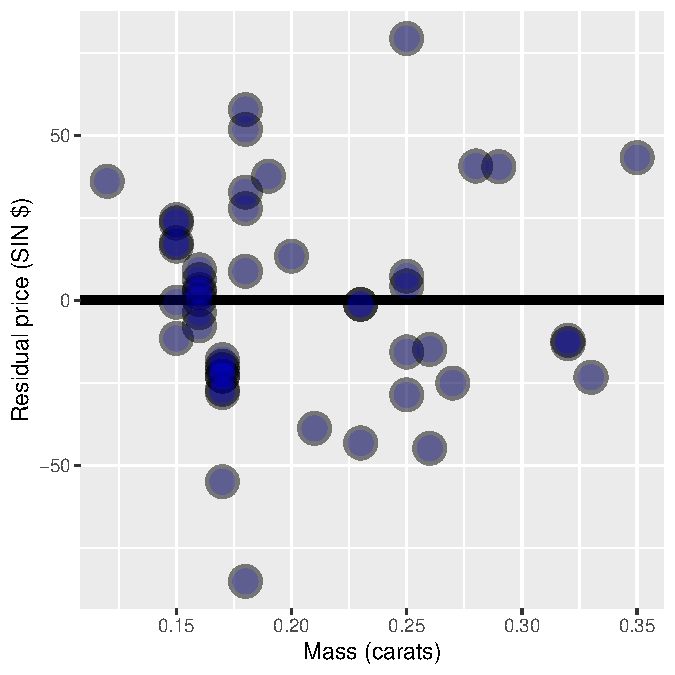
\includegraphics{semana_4_files/figure-latex/unnamed-chunk-13-1} \end{center}

Ejemplo de descomposición de series de tiempo

\begin{itemize}
\tightlist
\item
  \textbf{Tendencia}: patrón en constante aumento a lo largo del tiempo
\item
  \textbf{estacional}: cuando hay un patrón durante un período de tiempo
  fijo que se repite.
\item
  \textbf{ciclo}: cuando los datos aumentan y disminuyen durante
  períodos no fijos \url{https://www.otexts.org/fpp/6/1}
\end{itemize}

\begin{Shaded}
\begin{Highlighting}[]
\FunctionTok{plot}\NormalTok{(}\FunctionTok{decompose}\NormalTok{(ts1),}\AttributeTok{xlab=}\StringTok{"Years+1"}\NormalTok{)}
\end{Highlighting}
\end{Shaded}

\begin{center}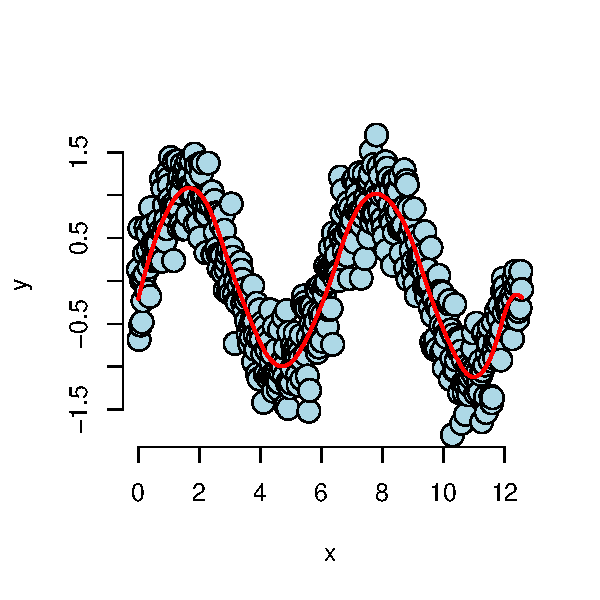
\includegraphics{semana_4_files/figure-latex/unnamed-chunk-14-1} \end{center}

creando conjuntos de prueba y de entrenamiento

\begin{Shaded}
\begin{Highlighting}[]
\NormalTok{ts1Train }\OtherTok{\textless{}{-}} \FunctionTok{window}\NormalTok{(ts1,}\AttributeTok{start=}\DecValTok{1}\NormalTok{,}\AttributeTok{end=}\DecValTok{5}\NormalTok{)}
\NormalTok{ts1Test }\OtherTok{\textless{}{-}} \FunctionTok{window}\NormalTok{(ts1,}\AttributeTok{start=}\DecValTok{5}\NormalTok{,}\AttributeTok{end=}\NormalTok{(}\DecValTok{7}\FloatTok{{-}0.01}\NormalTok{))}
\NormalTok{ts1Train}
\end{Highlighting}
\end{Shaded}

\begin{verbatim}
##        Jan      Feb      Mar      Apr      May      Jun      Jul      Aug
## 1 345.1413 263.3479 234.8746 223.0340 288.0752 290.1624 258.8199 235.3728
## 2 153.7238 166.5208 166.0426 171.2481 196.7774 208.5832 211.3080 223.5322
## 3 312.3044 266.3018 263.6119 284.6082 262.2670 239.3180 221.8136 243.5820
## 4 297.1263 301.1163 307.7365 293.2807 271.8311 263.0341 252.4239 304.4688
## 5 325.2509                                                               
##        Sep      Oct      Nov      Dec
## 1 237.4948 204.8073 178.1224 142.8047
## 2 228.9817 245.5795 267.5372 292.9669
## 3 226.6405 264.0104 306.7154 280.4488
## 4 269.3654 253.9731 288.9669 298.8797
## 5
\end{verbatim}

medias moviles simples

\[ Y_{t}=\frac{1}{2*k+1}\sum_{j=-k}^k {y_{t+j}}\]

\begin{Shaded}
\begin{Highlighting}[]
\FunctionTok{library}\NormalTok{(forecast)}
\FunctionTok{plot}\NormalTok{(ts1Train)}
\FunctionTok{lines}\NormalTok{(}\FunctionTok{ma}\NormalTok{(ts1Train,}\AttributeTok{order=}\DecValTok{3}\NormalTok{),}\AttributeTok{col=}\StringTok{"red"}\NormalTok{)}
\end{Highlighting}
\end{Shaded}

\begin{center}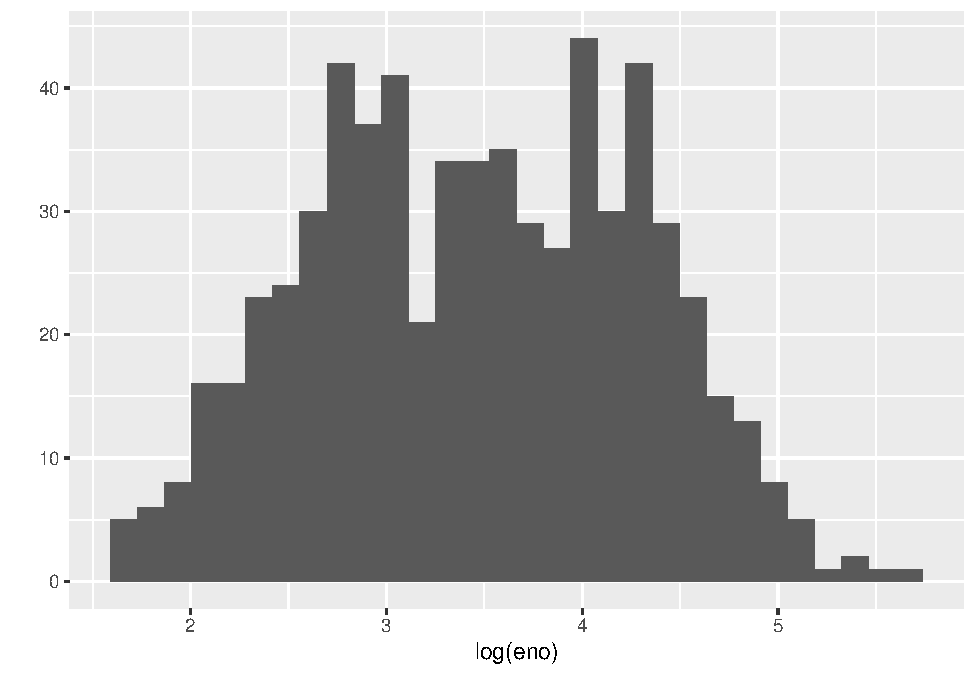
\includegraphics{semana_4_files/figure-latex/unnamed-chunk-16-1} \end{center}

suavizado exponencial

\[\hat{y}_{t+1} = \alpha y_t + (1-\alpha)\hat{y}_{t-1}\]

\begin{center}\includegraphics[width=1\linewidth]{D:/luism/Documents/courses/assets/img/08_PredictionAndMachineLearning/extrapolation} \end{center}

\begin{Shaded}
\begin{Highlighting}[]
\CommentTok{\#ets1 \textless{}{-} ets(ts1Train,model="MMM")}
\CommentTok{\#fcast \textless{}{-} forecast(ets1)}
\CommentTok{\#plot(fcast); lines(ts1Test,col="red")}
\end{Highlighting}
\end{Shaded}

obteniendo la precision

\begin{Shaded}
\begin{Highlighting}[]
\CommentTok{\#accuracy(fcast,ts1Test)}
\end{Highlighting}
\end{Shaded}

\hypertarget{notas-y-otros-recursos-1}{%
\subsection{Notas y otros recursos}\label{notas-y-otros-recursos-1}}

\begin{itemize}
\tightlist
\item
  \href{http://en.wikipedia.org/wiki/Forecasting}{Pronóstico y
  predicción de series temporales} es un campo completo
\item
  Rob Hyndman \href{https://www.otexts.org/fpp/}{Pronóstico: principios
  y práctica} es un buen lugar para comenzar
\item
  Precauciones

  \begin{itemize}
  \tightlist
  \item
    Tenga cuidado con las correlaciones falsas
  \item
    Tenga cuidado con lo lejos que predice (extrapolación)
  \item
    Tenga cuidado con las dependencias a lo largo del tiempo
  \end{itemize}
\item
  Ver paquetes de
  \href{http://cran.r-project.org/web/packages/quantmod/quantmod.pdf}{quantmod}
  o {[}quandl{]} (\url{http://www.quandl.com/help/packages/r}) para
  problemas relacionados con las finanzas.
\end{itemize}

\hypertarget{prediccion-sin-supervision}{%
\section{prediccion sin supervision}\label{prediccion-sin-supervision}}

Ideas claves

\begin{itemize}
\tightlist
\item
  A veces no conoce las etiquetas para la predicción
\item
  Para construir un predictor

  \begin{itemize}
  \tightlist
  \item
    Crear clústeres
  \item
    nombrar lis clústeres
  \item
    Construir predictor para clústeres
  \end{itemize}
\item
  En un nuevo conjunto de datos

  \begin{itemize}
  \tightlist
  \item
    Predecir clústeres
  \end{itemize}
\end{itemize}

Ejemplo de iris ignorando las etiquetas de las especies

\begin{Shaded}
\begin{Highlighting}[]
\FunctionTok{data}\NormalTok{(iris); }\FunctionTok{library}\NormalTok{(ggplot2)}
\NormalTok{inTrain }\OtherTok{\textless{}{-}} \FunctionTok{createDataPartition}\NormalTok{(}\AttributeTok{y=}\NormalTok{iris}\SpecialCharTok{$}\NormalTok{Species,}
                              \AttributeTok{p=}\FloatTok{0.7}\NormalTok{, }\AttributeTok{list=}\ConstantTok{FALSE}\NormalTok{)}
\NormalTok{training }\OtherTok{\textless{}{-}}\NormalTok{ iris[inTrain,]}
\NormalTok{testing }\OtherTok{\textless{}{-}}\NormalTok{ iris[}\SpecialCharTok{{-}}\NormalTok{inTrain,]}
\FunctionTok{dim}\NormalTok{(training); }\FunctionTok{dim}\NormalTok{(testing)}
\end{Highlighting}
\end{Shaded}

\begin{verbatim}
## [1] 105   5
\end{verbatim}

\begin{verbatim}
## [1] 45  5
\end{verbatim}

en el siguiente dendograma vemos que con una distancia de 3.5 podemos
crear 3 grupos

\begin{Shaded}
\begin{Highlighting}[]
\NormalTok{distra}\OtherTok{\textless{}{-}}\FunctionTok{dist}\NormalTok{(}\FunctionTok{subset}\NormalTok{(training,}\AttributeTok{select=}\SpecialCharTok{{-}}\FunctionTok{c}\NormalTok{(Species)))}
\NormalTok{hc}\OtherTok{\textless{}{-}}\FunctionTok{hclust}\NormalTok{(distra)}
\FunctionTok{plot}\NormalTok{(hc)}
\end{Highlighting}
\end{Shaded}

\begin{center}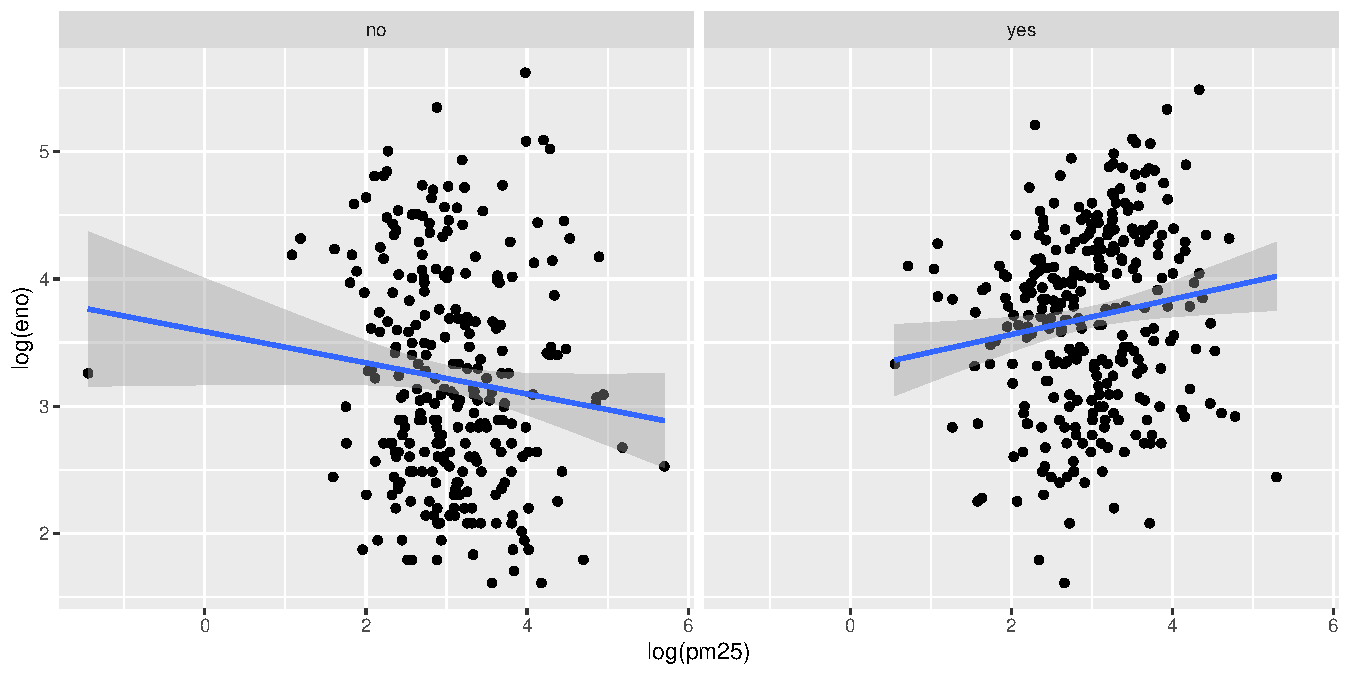
\includegraphics{semana_4_files/figure-latex/unnamed-chunk-21-1} \end{center}

ahora creemos 3 grpos con k-means

\begin{Shaded}
\begin{Highlighting}[]
\NormalTok{kMeans1 }\OtherTok{\textless{}{-}} \FunctionTok{kmeans}\NormalTok{(}\FunctionTok{subset}\NormalTok{(training,}\AttributeTok{select=}\SpecialCharTok{{-}}\FunctionTok{c}\NormalTok{(Species)),}\AttributeTok{centers=}\DecValTok{3}\NormalTok{)}
\NormalTok{training}\SpecialCharTok{$}\NormalTok{clusters }\OtherTok{\textless{}{-}} \FunctionTok{as.factor}\NormalTok{(kMeans1}\SpecialCharTok{$}\NormalTok{cluster)}
\FunctionTok{qplot}\NormalTok{(Petal.Width,Petal.Length,}\AttributeTok{colour=}\NormalTok{clusters,}\AttributeTok{data=}\NormalTok{training)}
\end{Highlighting}
\end{Shaded}

\begin{center}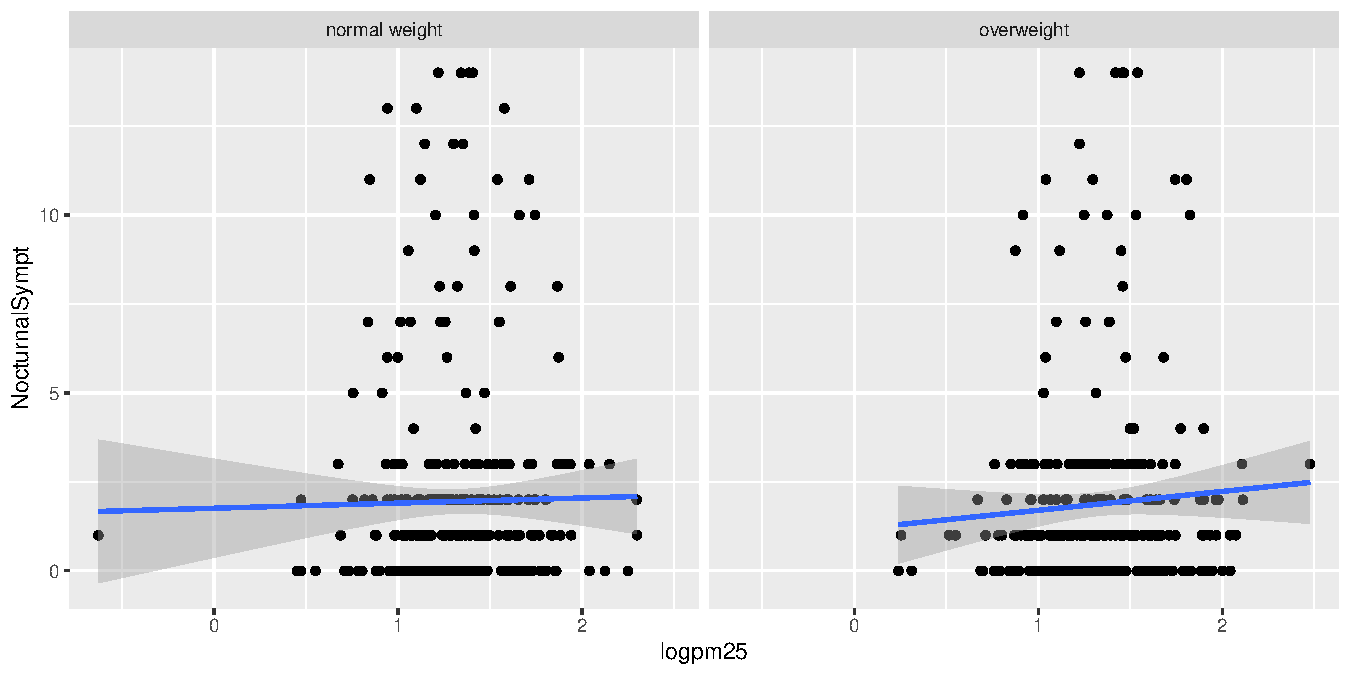
\includegraphics{semana_4_files/figure-latex/unnamed-chunk-22-1} \end{center}

comparando con las etiquetas reales

\begin{Shaded}
\begin{Highlighting}[]
\FunctionTok{table}\NormalTok{(kMeans1}\SpecialCharTok{$}\NormalTok{cluster,training}\SpecialCharTok{$}\NormalTok{Species)}
\end{Highlighting}
\end{Shaded}

\begin{verbatim}
##    
##     setosa versicolor virginica
##   1     35          0         0
##   2      0          2        26
##   3      0         33         9
\end{verbatim}

construyendo un predictor

\begin{Shaded}
\begin{Highlighting}[]
\NormalTok{modFit }\OtherTok{\textless{}{-}} \FunctionTok{train}\NormalTok{(clusters }\SpecialCharTok{\textasciitilde{}}\NormalTok{.,}\AttributeTok{data=}\FunctionTok{subset}\NormalTok{(training,}\AttributeTok{select=}\SpecialCharTok{{-}}\FunctionTok{c}\NormalTok{(Species)),}\AttributeTok{method=}\StringTok{"rpart"}\NormalTok{)}
\FunctionTok{table}\NormalTok{(}\FunctionTok{predict}\NormalTok{(modFit,training),training}\SpecialCharTok{$}\NormalTok{Species)}
\end{Highlighting}
\end{Shaded}

\begin{verbatim}
##    
##     setosa versicolor virginica
##   1     35          0         0
##   2      0          0        25
##   3      0         35        10
\end{verbatim}

aplicando en el conjunto de prueba

\begin{Shaded}
\begin{Highlighting}[]
\NormalTok{testClusterPred }\OtherTok{\textless{}{-}} \FunctionTok{predict}\NormalTok{(modFit,testing) }
\FunctionTok{table}\NormalTok{(testClusterPred ,testing}\SpecialCharTok{$}\NormalTok{Species)}
\end{Highlighting}
\end{Shaded}

\begin{verbatim}
##                
## testClusterPred setosa versicolor virginica
##               1     15          0         0
##               2      0          0         9
##               3      0         15         6
\end{verbatim}

\hypertarget{notas-y-lectura-adicional}{%
\subsection{Notas y lectura adicional}\label{notas-y-lectura-adicional}}

\begin{itemize}
\tightlist
\item
  La función cl\_predict en el paquete clue proporciona una
  funcionalidad similar
\item
  ¡Tenga cuidado con la interpretación excesiva de los grupos!
\item
  Este es un enfoque básico para
  \href{http://en.wikipedia.org/wiki/Recommender_system}{motores de
  recomendación}
\item
  \href{http://www-stat.stanford.edu/~tibs/ElemStatLearn/}{Elementos del
  aprendizaje estadístico}
\item
  \href{http://www-bcf.usc.edu/~gareth/ISL/}{Introducción al aprendizaje
  estadístico}
\end{itemize}

\end{document}
